\section{TypeScript}
\label{typescript}

\textit{TypeScript} ist eine 2012 erschienene Programmiersprache, welche von Microsoft entwickelt wurde und \textit{\nameref{javascript}} ein Typensystem hinzufügt. Ansonsten basiert TypeScript vollständig auf JavaScript und lässt sich deshalb auch zu JavaScript kompilieren.

\begin{code}[htp]
    \begin{center}
        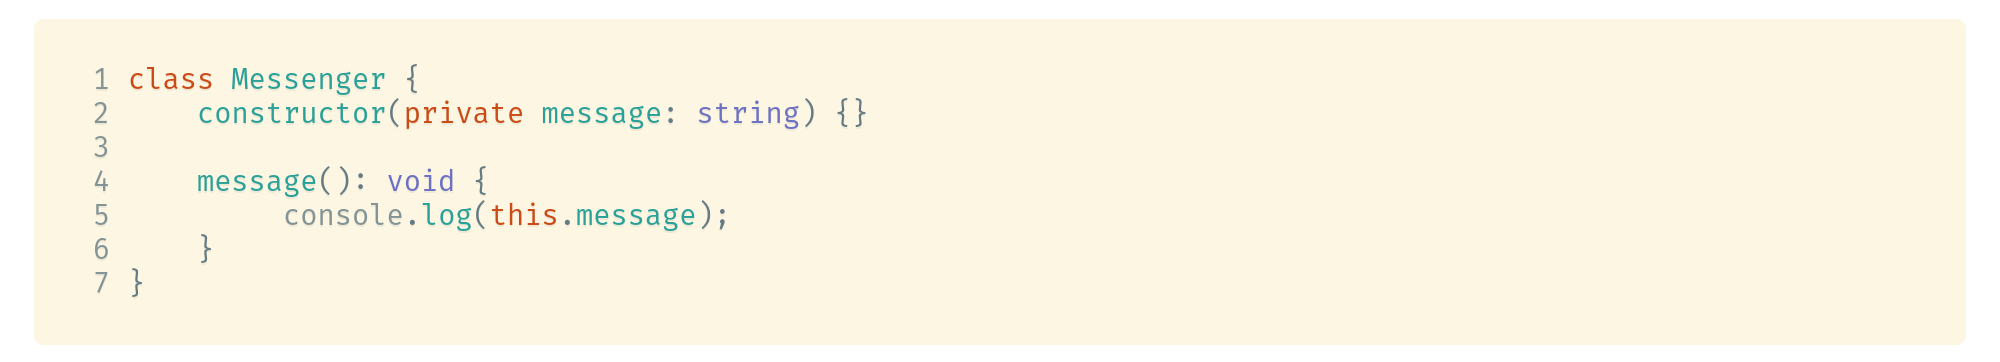
\includegraphics[width=1\textwidth]{images/TypeScript/TS.png}
        \vspace{-25pt}
        \caption{Eine Klasse mit einer einfachen Funktion in TypeScript}
    \end{center}
\end{code}

\begin{code}[htp]
    \begin{center}
        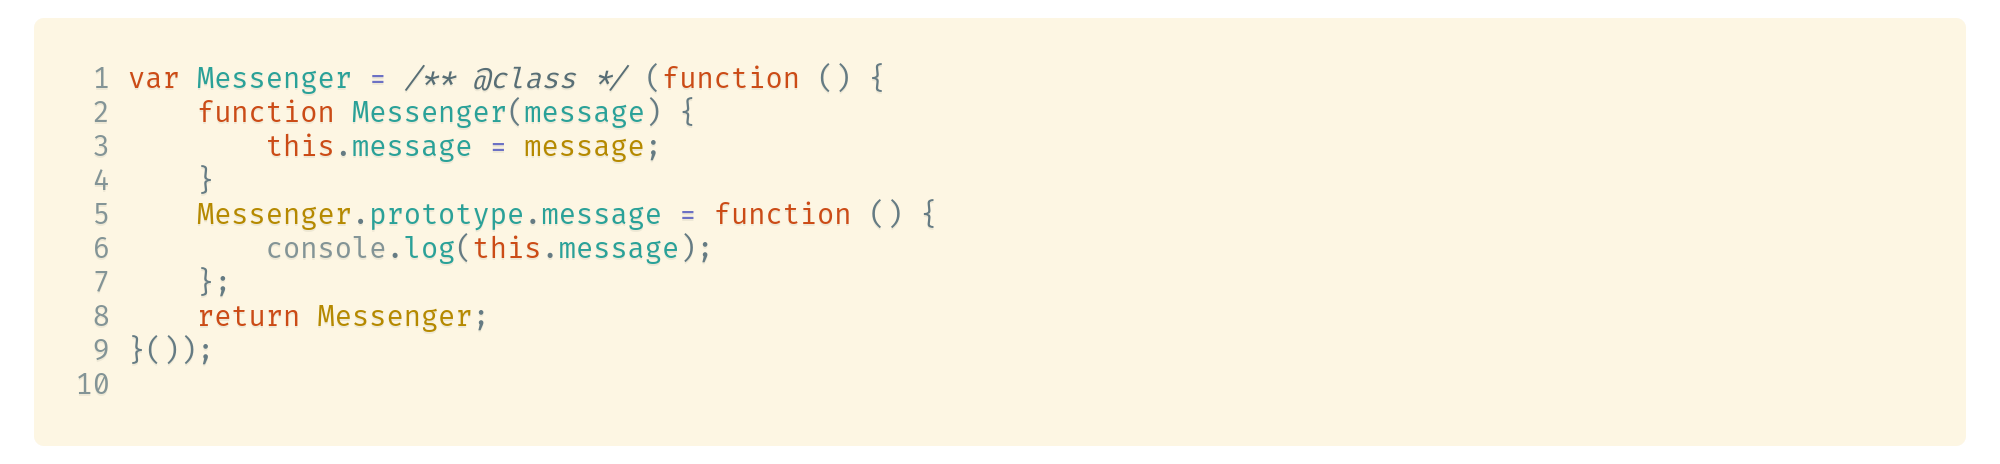
\includegraphics[width=1\textwidth]{images/TypeScript/JS.png}
        \vspace{-25pt}
        \caption{Eine von TypeScript zu JavaScript konvertierte Klasse}
    \end{center}
\end{code}

In Sokka wird TypeScript sowohl als primäre Programmiersprache für das \nameref{backend}, als auch als Programmiersprache für das \nameref{acp} verwendet.